136. \begin{figure}[ht!]
\center{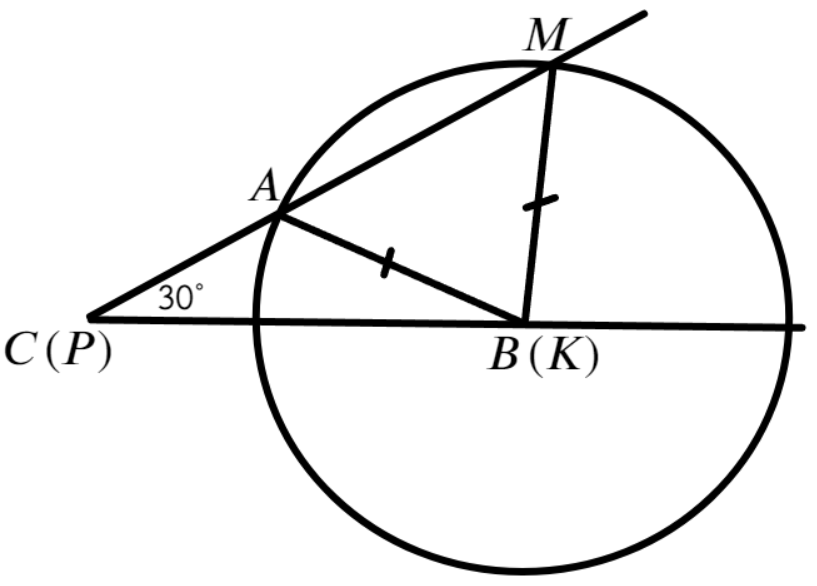
\includegraphics[scale=0.35]{g7-136.png}}
\end{figure}\\
Нет, они могут быть не равны. Построим контрпример: совместим углы $C$ и $P,$ на одной из сторон отложим $CB=PK=4.$ После этого построим окружность с центром в точке $B(K)$ и радиусом 3, пусть она пересечёт вторую сторону угла в точках $A$ и $M.$ Тогда в треугольниках $ABC$ и $MKP$ выполняются все данные условия, но они не равны.\\
